\documentclass{cours}
\usepackage{pgfplots}
\usepackage{multicol}
\usepackage{calc}
\usepackage{esvect}
\usepackage{tikz-3dplot} 
\usetikzlibrary{patterns}
\usetikzlibrary{decorations.text}
\begin{document}
\setcounter{chapter}{10}
\chapter{Dynamique newtonienne}
\begin{minipage}{7cm}
\begin{center}
  \includegraphics[width=5cm]{images/newton.jpg}
\end{center}
\end{minipage}%
\begin{minipage}{\linewidth - 7cm}
  Isaac \textsc{Newton} (1642 -- 1727), physicien, mathématicien, astronome, alchimiste et philosophe anglais. Il a fondé la mécanique classique, établit la loi de la gravitation universelle, développé le calcul infinitésimal (dérivation, intégration), développé une théorie de la couleur et inventé le télescope à miroir concave.  
\end{minipage}
\section{Les force}%
\label{sec:les_force}

Une force est une action d'un objet sur un autre, induisant une accélération de ce dernier. Une force est modélisée par un vecteur $\vv{F}$. L'intensité d'une force est en newtons (N).

\subsection{Loi des actions réciproques -- troisième loi de Newton}%
\label{sub:loi_des_actions_reciproques}

Lorsqu'un objet $A$ exerce sur un objet $B$ une force $\vv*{F}{A\rightarrow B}$, l'objet $B$ exerce sur $A$ une force opposée 
\begin{equation}
\vv*{F}{B\rightarrow A} = - \vv*{F}{A\rightarrow B}
\end{equation}

\begin{center}
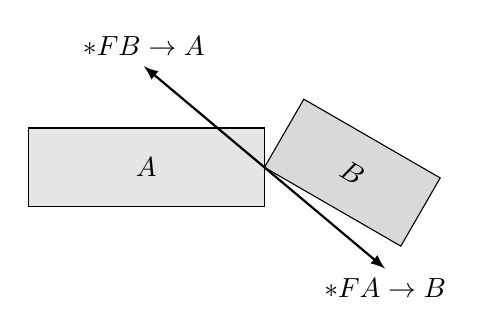
\begin{tikzpicture}
  \draw[fill=gray!20] (0,0) rectangle (3,1) node[midway] {$A$}; 
  \draw[rotate around={-30:(3, 0.5)}, fill=gray!30] (3,0.5) rectangle ++(2,1) node[midway, rotate=-30] {$B$}; 
  \draw[thick, -latex](3, 0.5) -- ++(140:2) node[above]{$\vv*{F}{B\rightarrow A}$ };
  \draw[thick, -latex](3, 0.5) -- ++(140:-2) node[below]{$\vv*{F}{A\rightarrow B}$ };
\end{tikzpicture}
\end{center}

\subsection{Quelques forces usuelles}%
\subsubsection{Forces de frottement fluide}%
\label{ssub:forces_de_frottement_fluide}

Un objet qui se déplace à la vitesse $\vv{v}$ dans un fluide est soumis à une force de frottement opposée à $\vv{v}$. 

À faible vitesse (écoulement laminaire), on a :
\begin{eqencadre}
\vv{f} = -k \vv{v}
\end{eqencadre}
où $k$ dépend de la forme de l'objet et de la viscosité du fluide. 

À haute vitesse (écoulement turbulent) :
\begin{eqencadre}
\norm{\vv{f}} = kv^2
\end{eqencadre}

\subsubsection{Forces de frottement solide}%

Lorsqu'un solide $A$ est en contact avec un autre solide $B$, le solide $B$ exerce sur $A$ une force $F$ que l'on peut décomposer en deux composantes :
\begin{itemize}
  \item Une composante tangentielle à l'interface entre les deux solides $\vv{T}$;
  \item une composante normale à l'interface $\vv{N}$. 
\end{itemize}

\begin{center}
  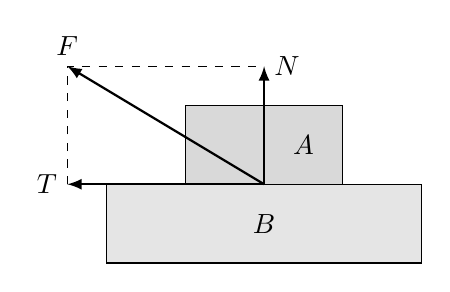
\begin{tikzpicture}
    \draw[fill=gray!20] (0,0) rectangle (4,1) node[midway]{$B$};
    \draw[fill=gray!30] (1,1) rectangle (3,2) node[midway, xshift=0.5cm]{$A$};
    \draw[-latex, thick] (2,1) coordinate (M) -- ++(0,1.5) node[right]{$\vv{N}$};  
    \draw[-latex, thick] (M) -- ++(-2.5, 0) node[left]{$\vv{T}$}; 
    \draw[-latex, thick] (M) -- ++(-2.5, 1.5) node[above]{$\vv{F}$}; 
    \draw[dashed](M) ++(-2.5, 0) -- ++(0, 1.5) -- ++(2.5, 0);

  \end{tikzpicture}
\end{center}

\subsubsection{Le poids}%
\label{ssub:le_poids}

La force d'attraction gravitationnelle exercée par la Terre sur un objet proche de la surface est 
\begin{eqencadre}
\vv{P} = m \vv{g} \quad \text{avec}\quad \norm{\vv{g}} = \SI{9.8}{\newton\per\kilo\gram}
\end{eqencadre}

Lorsque l'on considère des mouvements sur une échelle qui devient de l'ordre de la taille de la Terre, il faut considérer la force de gravitation exercée par la Terre sur le point $M$ :
\begin{eqencadre}
\vv{F}_{T\rightarrow M} = -G\frac{m_Tm}{r^2}\ver
\end{eqencadre}
où $r$ est la distance entre le centre de la Terre et le point $M$ et $\ver$ est un vecteur unitaire orienté du centre de la Terre vers le point $M$. 

\subsubsection{Force de rappel d'un ressort}%
\label{ssub:force_de_rappel_d_un_ressort}

Un ressort exerce sur un objet une force proportionnelle à son élongation $\delta \vv{x}$ : 
\begin{center}
\begin{tikzpicture}
  %tikz meca
%mur
\draw (0,-1) -- (0,1);
\foreach \h in {-1,-0.8,...,1} {
  \draw (0,\h) -- ($(-0.3,\h-0.3)$);
}
%axe
\draw[->] (0,-0.5) -- (10,-0.5) node[above] {$\vec{e}_x$};
\draw[decorate,decoration={zigzag,amplitude=0.3cm,pre length=0.5cm,post length=0.5cm}] (0,0.1) -- (5,0.1);

\draw[thick,rounded corners=1mm] (5,0.7) rectangle (6.2,-0.45) node[midway] {$m$};
\draw[thick,rounded corners=1mm, opacity=0.3] (3.4,0.7) rectangle (4.6,-0.45) node[midway] {$m$};
\draw[dotted] (5.6,-0.45) -- (5.6,-1);
\draw[dotted] (4,0.5) -- (4,-1);
\draw[-latex] (4,-1) -- (5.6,-1) node[midway,fill=white] {$\delta\vv{x}$};
\draw[->,coul1,thick] (5,0.1) -- (3.5,0.1) node[above,fill=white,opacity=0.6,text opacity=1,yshift=3] {$\vec{F}$};
\draw (2,1) node[align=center] {$k$};
%\draw[<-] (4,-1) to[bend left] (3.5,-1.2) node[left,align=center] {Position \\d'équilibre};
\draw[latex-latex] (0, -1) -- (4, -1) node[midway, below, align=center]{Longueur\\à vide : $\ell_0$ };
\end{tikzpicture}
\end{center}
\begin{eqencadre}
\vv{F} = -k\delta \vv{x}
\end{eqencadre}
(Voir fiche d'entraînement technique sur les ressorts)
\subsubsection{Poussée d'Archimède}%
\label{ssub:poussee_d_archimede}
Un objet $A$ de volume $V$ plongé dans un fluide de masse volumique $\rho$ est soumis à une force opposée à son poids 
\begin{eqencadre}
\vv*{F}{A} = -\rho V \vv{g}
\end{eqencadre}
\begin{center}
  \begin{tikzpicture}
    \draw[fill=gray!30] (-2,-1) rectangle (2,1);
    \draw[fill=white] (0,0) circle (0.6);
    \draw[<-] (0.2, 0) -- (3, 0.8) node[right]{Objet};
    \draw[<-] (-1.2, 0) -- (-3, 0.8) node[left]{Fluide};
    \draw[coul1, -latex, thick] (0,0) -- ++(0, 1.5) node[right]{$\vv*{F}{A}$}; 
    \draw[coul1, -latex, thick] (0,0) -- ++(0, -1.5) node[right]{$\vv{P}$}; 
    \draw[fill] (0,0) circle(2pt);
  \end{tikzpicture}
\end{center}
La force s'applique au centre de masse du fluide déplacé. Si l'objet n'est pas entièrement immergé, le volume $V$ est le volume immergé.

\section{Les lois du mouvement}%
\label{sec:les_lois_du_mouvement}

\subsection{Quantité de mouvement}%
\label{sub:quantite_de_mouvement}

\begin{definition}
  La quantité de mouvement $\vv{p}$ d'un point matériel de masse $m$ animé d'une vitesse $\vv{v}$ dans le référentiel d'étude $\mathcal{R}$ est 
  \begin{equation}
  \vv{p} = m \vv{v}
  \end{equation}
 C'est une grandeur qui dépend du référentiel choisi.
\end{definition}

On peut également définir la quantité de mouvement d'un ensemble de points $M_i$ comme la somme des quantités de mouvement de chaque point :
\begin{equation}
\vv{p} = \sum_i \vv*{p}{i} = \sum_i m_i \vv*{v}{i} = \sum_i m_i \dt{\vv{OM_i}} = \dt{}\left( \sum_i m_i \vv{OM_i} \right) 
\end{equation}

On définit le \emph{centre de gravité} $G$ du système de points comme le barycentre des points pondérés par leur masse :
\begin{equation}
m_t \vv{OG} = \sum_i m_i \vv{OM_i} 
\end{equation}
où $m_t = \sum_i m_i$ est la masse totale du système.

On en déduit que la quantité de mouvement du système de points matériels s'exprime comme :
\begin{equation}
\vv{p} = m_t  \dt{\vv{OG}} = m_t \vv*{v}{G}
\end{equation}
Pour la quantité de mouvement, tout se passe comme si toute la masse du système était concentrée au point $G$. 

\subsection{Référentiels galiléens -- première loi de Newton }%
\label{sub:referentiels_galileens}
\begin{definition}
Parmi tous les référentiels possibles, il existe une famille de référentiels par rapport auxquels un point matériel isolé (soumis à aucune force) est soit au repos, soit animé d'un mouvement rectiligne uniforme.

Ce sont les \textbf{référentiels galiléens} 
\end{definition}

Tout référentiel en translation rectiligne uniforme par rapport à un référentiel galiléen est également galiléen.

\subsection{Principe fondamental de la dynamique -- deuxième loi de Newton}%
\label{sub:principe_fondamental_de_la_dynamique_deuxieme_loi_de_newton}

Dans un référentiel galiléen, la variation $\dt{\vv{p}}$ de la quantité de mouvement d'un point matériel est égale à la somme des forces appliquées à ce point :
\begin{equation}
\dt{\vv{p}} = \sum_i \vv*{F}{i}
\end{equation}
Comme la masse d'un point matériel est constante, on écrit souvent cette relation sous la forme
\begin{equation}
m \vv{a} = \sum_i \vv*{F}{i}
\end{equation}
où $\vv{a}$ est l'accélération du point matériel dans le référentiel d'étude.

Pour un système de points matériels, de centre de gravité $G$, cette relation devient 
\begin{equation}
m_t \vv*{a}{G} = \sum_i \vv*{F}{i}^\text{ext}
\end{equation}
où $m_t$ est la masse totale du système de points matériels et les $\vv*{F}{i}^\text{ext}$ sont les forces dont l'origine est extérieure au système. En effet, d'après la loi des actions réciproques, les forces intérieures s'annulent deux à deux. 

\section{Applications}%
\label{sec:applications}

\subsection{Mouvement dans le champ de pesanteur terrestre}%
\label{sub:mouvement_dans_le_champ_de_pesanteur_terrestre}
On considère un point matériel $M$ de masse $m$ soumis uniquement à son poids $\vv{P} = m\vv{g}$.

\begin{center}
  \begin{tikzpicture}
    \draw[-latex] (0,0) coordinate (O) -- ++(2,0,0) node[right]{$\vey$} ;
    \draw[-latex] (O) -- ++(0,2,0) node[left]{$\vez$} ;
    \draw[-latex] (O) -- ++(0,0,2) node[left]{$\vex$} ;
    \fill (0.5, 1, 0.2) coordinate (M) circle(2pt); 
    \draw[-latex, thick] (M) -- ++(0, -1.3,0) node[midway, right]{$\vv{P}$}; 

  \end{tikzpicture}
\end{center}

Le principe fondamental de la dynamique appliqué au point $M$ dans le référentiel du laboratoire supposé galiléen donne :
\begin{equation}
m \vv{a} = m \vv{g} \Leftrightarrow \vv{a} = \vv{g}
\end{equation}
On a donc un mouvement de vecteur accélération constant. On a montré dans le chapitre précédent que le mouvement est rectiligne uniforme dans le plan $(x, y)$ et uniformément accéléré suivant l'axe $z$. La trajectoire est parabolique.

\subsection{Influence des frottements fluides}%
\label{sub:influence_des_frottements_fluides}
On s'intéresse à la chute verticale d'un objet soumis à son poids, avec et sans frottements de l'air. 

\subsubsection{Sans frottements}%
\label{ssub:sans_frottements}

\begin{center}
  \begin{tikzpicture}
    \draw (0,0) coordinate (O);
    \draw[-latex] (O) -- ++(0,2,0) node[left]{$\vez$} ;
    \fill (0.5, 1) coordinate (M) circle(2pt); 
    \draw[-latex, thick] (M) -- ++(0, -1.3,0) node[midway, right]{$\vv{P}$}; 

  \end{tikzpicture}
\end{center}
Comme dans l'exemple précédent, on applique le principe fondamental de la dynamique pour obtenir
\begin{equation}
m \vv{a} = m \vv{g} \Leftrightarrow \vv{a} = \vv{g} = -g\vez
\end{equation}
Or $\vv{a} = \ddot{z}\vez$, donc on a 
\begin{equation}
\ddot{z} = -g \Leftrightarrow \dot{z} = -gt + v_{0z} \Leftrightarrow z(t) = -\frac{1}{2}gt^2 + v_{0z}t + z_0 
\end{equation}
On peut représenter l'évolution temporelle de $z(t)$ et $\dot{z}(t)$ :
\begin{center}
  \begin{tikzpicture}
    %tikz meca
    \begin{axis}[
    xlabel=$t$ (s),
    ylabel=$z(t)$ (m),
    xmin=0,
    ymin=0,
    ]
      \addplot[domain=0:4.5, thick] {-0.5*9.881*x^2+100};
    \end{axis}
  \end{tikzpicture}
  \hspace{1em}
  \begin{tikzpicture}
    \begin{axis}[
    xlabel=$t$ (s),
    ylabel=$\dot{z}(t)$ (m/s),
    xmin=0,
    ]
      \addplot[domain=0:4.5, thick] {-9.881*x};
    \end{axis}
  \end{tikzpicture}
\end{center}

\subsubsection{Avec les frottements de l'air}%
\label{ssub:avec_les_frottements_de_l_air}
On considère maintenant que le point matériel subit une force de frottement fluide $\vv{f}$ opposée à sa vitesse, de norme  $\norm{\vv{f}} = k v^2$. On considère qu'il est lâché sans vitesse initiale, il va donc acquérir une vitesse suivant l'axe $\vez$. Le principe fondamental de la dynamique devient 
\begin{equation}
m \vv{a} = m \ddot{z}\vez  = \vv{P} + \vv{f} = -mg\vez + k \dot{z}^2 \vez
\end{equation}
On obtient donc l'équation différentielle 
\begin{equation}
\ddot{z} - \frac{k}{m}\dot{z}^2 = -g
\end{equation}
ou, si on note $v_z = \dot{z}$, on a :
\begin{equation}
\dot{v}_z - \frac{k}{m} v_z^2 = -g
\label{eq:diffv}
\end{equation}
C'est une équation différentielle non linéaire que l'on ne peut pas résoudre analytiquement. On peut néanmoins utiliser une méthode de résolution numérique pour obtenir $z(t)$ et $\dot{z}(t)$. La simulation suivante a été faite avec $k=\SI{0.02}{\newton\second\squared\per\meter\squared}$ et $m=\SI{1}{\kilo\gram}$. La courbe grise est celle obtenue sans les frottements. 
\begin{center}
  \begin{tikzpicture}
    \begin{axis}[
    xlabel=$t$ (s),
    ylabel=$z(t)$ (m),
    xmin=0,xmax=6,
    ymin=0,
    ]
      \addplot[thick] file {data_frottement.csv};
      \addplot[domain=0:4.5, thin, gray] {-0.5*9.881*x^2+100};
    \end{axis}
  \end{tikzpicture}
  \hspace{1em}
  \begin{tikzpicture}
    \begin{axis}[
    xlabel=$t$ (s),
    ylabel=$\dot{z}(t)$ (m/s),
    xmin=0,xmax=6,
    ]
      \addplot[thick] table[y index=2] {data_frottement.csv};
      \addplot[dashed, domain=0:6] {-22.136} node[pos=0.2, fill=white]{$v_\text{lim}$ };
      \addplot[domain=0:4.5, thin, gray] {-9.881*x};
    \end{axis}
  \end{tikzpicture}
\end{center}
On remarque que plus la vitesse augmente, plus l'accélération diminue. Si l'objet chute suffisamment longtemps, sa vitesse tend vers une vitesse limite $v_\text{lim}$ constante et son accélération tend vers 0.

On peut déterminer l'expression de $v_\text{lim}$ en prenant $\ddot{z}=0$ dans l'équation différentielle précédente, on trouve
\begin{equation}
\left|v_\text{lim}\right| = \sqrt{\frac{mg}{k}}
\label{eq:vlim}
\end{equation}

\subsubsection{Adimensionnement}%
\label{ssub:Adimensionnement}

On remarque que l'équation différentielle~\eqref{eq:diffv} fait intervenir 5 variables : $v_z$, $t$, $k$, $m$ et $g$. Or, on a montré que le système atteint une vitesse limite $v_\text{lim}$ donnée par l'équation~\eqref{eq:vlim}. Dans cette équation, on remarque, par exemple que si on double $m$ et $k$, alors la vitesse limite ne change pas et le mouvement devrait être très similaire. Il existe une \textbf{loi d'échelle} qui donne le même mouvement pour des valeurs de $m$ et $k$ différentes.

Pour rendre cette loi d'échelle plus évidente, on peut \textbf{adimensionner} l'équation~\ref{eq:diffv}. Pour cela, on va introduire des nouvelles grandeurs sans dimensions :
\begin{equation}
  v^* = \frac{v_z}{v_\text{lim}} \quad \text{et} \quad t^* = \frac{t}{\tau}
\end{equation}
où $\tau$ est un temps caractéristique dont on déterminera l'expression un peu plus tard.
La dérivation par rapport au temps $t$ devient
\begin{equation}
  \frac{\D}{\D t} = \frac{\D}{\D t^*}\dt{t^*} = \frac{1}{\tau}\frac{\D}{\D t^*}
\end{equation}
En effectuant les substitutions dans l'équation~\ref{eq:diffv}, on obtient:
\begin{equation}
  \frac{\D v^*}{\D t^*} \frac{v_\text{lim}}{\tau g} - {v^*}^2 = -1
\end{equation}

Le coefficient $\frac{v_\text{lim}}{\tau g}$ est sans dimension, et pour simplifier l'écriture de l'équation différentielle, on peut choisir $\tau=\frac{v_\text{lim}}{g}=\sqrt{\frac{m}{kg}}$. L'équation devient alors
\begin{equation}
  \frac{\D v^*}{\D t^*} - {v^*}^2 = -1
  \label{eq:diff_ad}
\end{equation}
Cette dernière équation ne fait intervenir que des grandeurs sans dimension, et lorsqu'on la compare avec l'équation~\eqref{eq:diffv}, on réalise qu'elle ne fait intervenir que 2 variables : $v^*$ et $t^*$. C'est une équation plus simple qui contient néanmoins toute la physique tu problème étudié. Si on trouve la solution de cette équation, on a directement la solution de n'importe quelle équation du type~\eqref{eq:diffv}. 

\subsection{Le pendule simple}%
\label{sub:le_pendule_simple}

Un pendule simple est composé d'une masse ponctuelle accrochée à l'extrémité d'un fil de longueur $l$. 
\begin{center}
  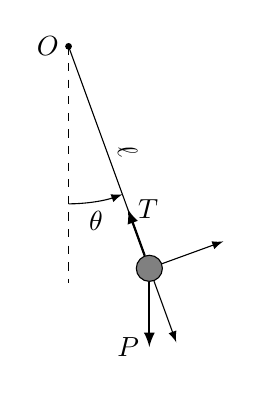
\begin{tikzpicture}
    %tikz meca
\draw[dashed] (0,0) -- (0,-3);
\draw[fill=black] (0,0) circle(1pt) coordinate (O) node[left]{$O$};
\draw (O) -- ++(-70:3) node[midway,above,sloped]{$\ell$} node[circle,fill=gray,draw=black,minimum height=0.1cm](M){};
%\draw (M.south) node[below]{$M(x,y)$};
\draw[-latex] (M) -- ++(20:1) node[right] {$\vet$}; 
\draw[-latex] (M) -- ++(-70:1) node[right] {$\ver$}; 
\draw[-latex, thick] (M) -- ++(-90:1) node[left] {$\vv{P}$}; 
\draw[-latex, thick] (M) -- ++(110:0.8) node[right] {$\vv{T}$}; 
\draw[-latex] (0,-2) arc (-90:-70:2) node[midway,below] {$\theta$};
  \end{tikzpicture}
\end{center}
La masse est soumise à son poids $\vv{P}$ et à la tension du fil $\vv{T}$. On cherche l'équation de son mouvement, donc $\theta(t)$. 

Le principe fondamental de la dynamique donne 
\begin{equation}
m \vv{a} = \vv{P} + \vv{T} = mg\cos(\theta)\ver - mg\sin(\theta)\vet -T\ver
\end{equation}

où $T = \norm{\vv{T}}$. 
Comme la masse est animée d'un mouvement circulaire, on a $\vv{a} = -\ell \dot{\theta}^2 + \ell \ddot{\theta} \vet$. En projetant le PFD sur l'axe $\vet$, on obtient l'équation :
\begin{equation}
\ell \ddot{\theta} + g\sin(\theta) = 0 \Leftrightarrow \ddot{\theta} + \frac{g}{\ell}\sin(\theta) = 0
\label{eq:pendule}
\end{equation}

Cette équation différentielle du second ordre n'est malheureusement pas linéaire et il n'est pas aisé de la résoudre analytiquement. Nous allons donc faire une approximation qui va nous permettre de la linéariser. Nous allons supposer que $\theta\ll 1$. Dans ces conditions $\sin(\theta) \approx \theta$ et on obtient l'équation 
\begin{equation}
\ddot{\theta} + \frac{g}{l} \theta = 0 \Leftrightarrow \ddot{\theta} + \omega_0^2 \theta = 0
\end{equation}

C'est l'équation d'un oscillateur harmonique ! Et nous connaissons sa solution : 
\begin{eqencadre}
\theta(t) = A\sin(\omega_0 t +\varphi)
\end{eqencadre}

On peut également intégrer l'équation~\ref{eq:pendule} numériquement pour voir les effets de la non-linéarité sur le comportement du pendule. Nous allons utiliser la fonction \texttt{solve\_ivp} de la bibliothèque \texttt{scipy.integrate}. 

Pour utiliser cette fonction avec une équation différentielle du deuxième ordre, il faut commencer par transformer l'équation différentielle en un système d'équations différentielles du premier ordre. On effectue cette transformation en posant 
\begin{equation}
  x_1 = \theta \quad \text{et} \quad  x_2 = \dot{\theta}
\end{equation}
On a alors le système d'équations suivant
\begin{equation}
  \begin{cases}
    \dot{x}_1 = x_2 \\
    \dot{x}_2 = -\omega_0^2\sin(x_1)
  \end{cases}
  \label{eq:systeme}
\end{equation}
En notant $X = \begin{pmatrix}x_1 \\ x_2\end{pmatrix}$ et $\dot{X} = \begin{pmatrix}\dot{x}_1\\\dot{x}_2\end{pmatrix}$, on peut écrire l'équation~\ref{eq:systeme} sous la forme
\begin{eqencadre}
  \dot{X} = F(X, t)
\end{eqencadre}

En pratique, cela devient
\begin{minted}{python}
import numpy as np
from scipy.integrate import solve_ivp
import matplotlib.pyplot as plt

def F(t, X):
  w0 = 1
  x1 = X[0]
  x2 = X[1]
  return [x2, -w0**2*np.sin(x1)]
 
X0 = [0.6, 0]                   # Conditions initiales
t  = [0, 20]                    # intervalle de temps (entre 0s et 10s)
tps = np.linspace(0, 20, 200)   # temps auxquels on veut la solution

# Résolution de l'équation
sol = solve_ivp(F, t, X0, t_eval = tps)  

plt.plot(sol['t'], sol['y'][0])           # affichage de la solution
plt.plot(sol['t'], 0.6*np.cos(sol['t']))  # solution de l'équation linéarisée
plt.show()
\end{minted}

On obtient alors les graphiques suivants :
\begin{center}
  \begin{tikzpicture}
    \begin{axis}[
      width=13cm, height=7cm,
      xmin=0, xmax=20,
      ymax=1,
      xlabel=Temps (s),
      ylabel=Angle (rad),
      ]
      \addplot[mark=none, smooth, thick] table[x index=0, y index=1] {data/pendule.csv};
      \addlegendentry{Solution numérique};
      \addplot[mark=none, smooth, thick, dashed] table[x index=0, y index=2] {data/pendule.csv};
      \addlegendentry{Solution de l'équation linéarisée};

    \end{axis}
  \end{tikzpicture}
\end{center}



%On peut alors calculer $\dot{\theta}(t)$ : 
%\begin{equation}
%\dot{\theta}(t) = A\omega_0\cos(\omega_0t + \varphi)
%\end{equation}

%et tracer le \emph{portrait de phase} de l'oscillateur :
%\begin{center}
  %\begin{tikzpicture}
    %\draw[-latex] (-2.5,0) -- (2.5,0) node[right]{$\theta$ };
    %\draw[-latex] (0,-2) -- (0,2) node[right]{$\dot{\theta}$ };
    %\draw[thick, postaction={decorate}, decoration={markings,mark=at position 1cm with{\arrowreversed{ stealth }}} ] (0,0) ellipse[x radius=2, y radius=1.5];

  %\end{tikzpicture}
%\end{center}

\section{Approche énergétique}%
\label{sec:approche_energetique}
\subsection{Travail et puissance d'une force}%
\label{sub:travail_et_puissance_d_une_force}

Le travail d'une force $\vv{F}$ appliquée à un point $M$ correspond à l'\emph{énergie} fournie à $M$ par la force $\vv{F}$ lors de son déplacement. Le travail s'exprime en joules.

Considérons un point $M$ de masse $m$ soumis à une force $\vv{F}$ et qui est déplacé d'un \emph{petit} vecteur $\D \vv{u}$ pour se retrouver en $M'$ . Comme le déplacement est très petit, il se fait en un temps $\D t$  très court et la vitesse du point $M$  change très peu. L'accélération $a$ du point $M$ est aussi quasiment constante. Nous allons déterminer l'énergie reçue par le point $M$ de la part de la force $\vv{F}$.  


\begin{center}
  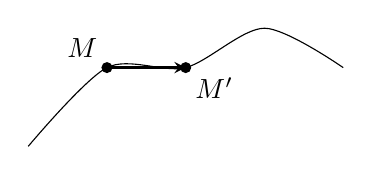
\begin{tikzpicture}
    \draw (1,1) coordinate(M) node[above left] {$M$} ; 
    \fill (1,1) circle(2pt);
    \fill (2,1) circle(2pt);
    \draw (2,1) coordinate (Mp) node[below right] {$M'$} ; 
    \draw[] plot[smooth] coordinates{(0,0)(1,1)(2,1)(3,1.5)(4,1)} ; 
    \draw[thick, -stealth] (M) -- (Mp);
    %\draw (0,0)--(2,0);
  \end{tikzpicture}
  \end{center}

L'énergie reçue par le point $M$ correspond à l'énergie cinétique gagnée entre $M$ et $M'$. Soit
\begin{equation}
  \Delta E_c = \frac{1}{2}mv_{M'}^2 - \frac{1}{2}mv_M^2 = \frac{1}{2}m\left( v_{M'}^2 - v_M^2 \right)   
\end{equation}

Comme le vecteur accélération est considéré comme constant sur ce trajet, on peut écrire 
\begin{equation}
  \vv*{v}{M'} = \vv*{v}{M} + \vv{a}\D t 
  \label{eq:vmp}
\end{equation}
%
Le principe fondamentale de la dynamique donne 
\begin{equation}
\vv{F} = m\vv{a}
\end{equation}
%
Et l'équation~\eqref{eq:vmp} devient 
\begin{equation}
  \vv*{v}{M'} = \vv*{v}{M} + \frac{\vv{F}}{m}\D t
\end{equation}
%
Et donc on a 
\begin{equation}
  v_{M'}^2 = \norm{\vv*{v}{M'}}^2 = \norm{\vv*{v}{M}}^2 + 2\frac{\vv{F}\cdot\vv*{v}{M}}{m}\D t + \underbrace{\frac{\norm{F}^2}{m^2}(\D t)^2}_{\text{négligé}}
\end{equation}

Comme $\D t$ est un temps arbitrairement petit, le terme en $(\D t)^2$ peut être négligé devant le terme en $\D t$. Et on obtient finalement
\begin{equation}
  \Delta E_c = \vv{F}\cdot\underbrace{\vv*{v}{M}\D t}_{=\D \vv{u}}
\end{equation}

Donc la variation d'énergie cinétique du point $M$ au cours de son déplacement est $\vv{F}\cdot\D\vv{u}$. Cette quantité est notée $\delta W$ est est appelée \emph{travail élémentaire} de la force $\vv{F}$.

\begin{eqencadre}
\delta W = \vv{F}\cdot\D\vv{u}
\end{eqencadre}

Pour déterminer le travail d'une force sur une trajectoire $\mathcal{C}$, il faut sommer tous les travaux élémentaires et on a : 
\begin{eqencadre}
W_\mathcal{C} = \int_\mathcal{C}\delta W = \int_\mathcal{C} \vv{F}\cdot\D \vv{u}
\end{eqencadre}

En particulier, si la force $\vv{F}$ est constante, on peut la sortir de l'intégrale et on obtient :
\begin{equation}
W_\mathcal{C} = \vv{F}\cdot\int_\mathcal{C}\D\vv{u} = \vv{F}\cdot\vv{AB}
\end{equation}
où $A$ et $B$ sont les points de départ et d'arrivée du chemin.
\begin{center}
  \begin{tikzpicture}
    \draw (0,0) node[below left] {$A$} ; 
    \fill (0,0) circle(2pt);
    \fill (4,1) circle(2pt);
    \draw (4,1) node[below right] {$B$} ; 
    \draw[thick, 
    postaction={decorate},
    decoration={
       post length=1mm,
       pre length=1mm,
       markings,
       mark=at position 0.3 with{\arrow{ stealth }}
    }
    ] 
    plot[smooth] coordinates{(0,0)(1,1)(2,1)(3,1.5)(4,1)}; 
    \draw (2,1) node[below]{$\mathcal{C}$} ;
    %\draw (0,0)--(2,0);
  \end{tikzpicture}
\end{center}

\begin{itemize}
  \item Si $W_\mathcal{C}>0$, la force fournit de l'énergie au point $M$, on dit que le travail est \textbf{moteur}.  
  \item Si $W_\mathcal{C}<0$, la force retire de l'énergie au point $M$, on dit que le travail est \textbf{résistant}. 
\end{itemize}



La puissance fournie par la force $\vv{F}$ est 
\begin{eqencadre}
P = \frac{\delta W}{\D t} = \vv{F}\cdot \dt{\vv{u}} = \vv{F}\cdot\vv{v}
  \end{eqencadre}

\subsection{Théorème de l'énergie cinétique}%
\label{sub:theoreme_de_l_energie_cinetique}

\begin{definition}
  L' \textbf{énergie cinétique} d'un point matériel $M$ de masse $m$ animé d'une vitesse $\vv{v}$ dans un référentiel $\mathcal{R}$ est
  \begin{equation}
  E_c = \frac{1}{2}mv^2
  \end{equation}
  
\end{definition}


Dans un référentiel galiléen, un point matériel $M$ de masse $m$ se déplace sur un chemin $\mathcal{C}$ entre les points $A$ et $B$. 
 
\begin{center}
  \begin{tikzpicture}
    \draw (0,0) node[below left] {$A$} ; 
    \fill (0,0) circle(2pt);
    \fill (4,1) circle(2pt);
    \draw (4,1) node[below right] {$B$} ; 
    \draw[thick, 
    postaction={decorate},
    decoration={
       post length=1mm,
       pre length=1mm,
       markings,
       mark=at position 0.3 with{\arrow{ stealth }};,
       mark=at position 0.5 with{\fill circle(2pt) node[below]{$M$};};,
    }
    ] 
    plot[smooth] coordinates{(0,0)(1,1)(2,1)(3,1.5)(4,1)}; 
    \draw (3,1.5) node[below]{$\mathcal{C}$} ;
    %\draw (0,0)--(2,0);
  \end{tikzpicture}
\end{center}

Dans ce cas, la variation d'énergie cinétique du point $M$ entre les points $A$ et $B$ est égale à la somme des travaux des forces appliquées à $M$ entre $A$ et $B$. 
\begin{eqencadre}
  \Delta E_c = E_c(B) - E_c(A) = \sum_i W_{A\rightarrow B} (\vv*{F}{i})
  \end{eqencadre}

Que l'on peut aussi en fonction des puissances :
\begin{eqencadre}
  \dt{E_c} = \sum_i P\left(\vv*{F}{i}\right) 
  \end{eqencadre}
Pour démontrer cette loi, on multiplie le PFD scalairement par $\vv{v}$ : 
\begin{align}
m \dt{\vv{v}}\cdot\vv{v} &= \sum_i \vv*{F}{i} \cdot \vv{v}\\
\frac{1}{2}m \dt{(\vv{v}\cdot\vv{v})} &= \sum_i P\left( \vv*{F}{i} \right)\\
\dt{}\underbrace{\left( \frac12m\norm{\vv{v}}^2 \right)}_{E_c} &= \sum_i P\left( \vv*{F}{i} \right)
\end{align}

\begin{application}
  Un objet de masse $m$ tombe d'une hauteur $h$ sans vitesse initiale, déterminer sa vitesse $v$  au moment de l'impact avec le sol (on néglige les frottements de l'air).
 
 On applique le théorème de l'énergie cinétique entre le début et la fin de la chute. L'énergie cinétique au début du mouvement est nulle et 
 \begin{equation}
 E_{cf} = \frac{1}{2}mv^2 = W_{A\rightarrow B}\left( \vv{P} \right) 
 \end{equation}
 Comme le poids $\vv{P}$ est constant sur le trajet $A\rightarrow B$, on a $W_{A\rightarrow B} = \vv{P}\cdot\vv{AB} = mgh$ 
 
 On obtient finalement 
 \begin{equation}
 v = \sqrt{2gh}
 \end{equation}
\end{application}


\subsection{Énergie potentielle est énergie mécanique}%
\label{sub:energie_potentielle_est_energie_mecanique}

\subsubsection{Énergie potentielle et force conservative}%
\label{ssub:energie_potentielle_est_force_conservative}

Considérons un point matériel $M$ soumis uniquement à son poids $\vv{P} = m\vv{g}$ entre $A$ et $B$. 

Le travail du poids entre les points $A$ et $B$ est 
\begin{equation}
W_{AB} = \int_A^B\vv{P}\cdot\D \vv{u} = \int_A^B m\vv{g}\cdot\D \vv{u} = m\vv{g}\cdot\int_A^B\D\vv{u} = m\vv{g}\cdot\vv{AB}
\end{equation}

Donc $W_{AB}$ est indépendant du chemin suivi entre $A$ et $B$. On dit que le poids est une \textbf{force conservative}.

On peut écrire $W_{AB}$ de la manière suivante :
\begin{center}
  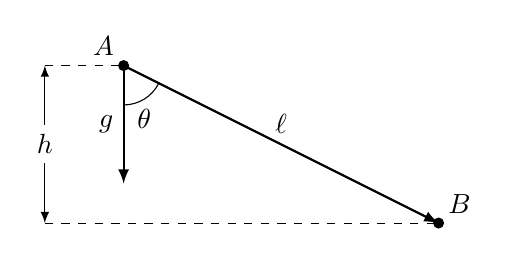
\begin{tikzpicture}
    \coordinate (A) at (0,0);
    \coordinate (B) at (4,-2);
    \fill (A) circle(2pt) node[above left] {$A$ };
    \fill (B) circle(2pt) node[above right] {$B$ };
    \draw[-latex, thick] (A) -- ++(0, -1.5) node[midway, left]{$\vv{g}$} ;
    \draw[-latex, thick] (A) --  (B) node[above, midway]{$\ell$} ;
    \draw (0, -0.5) arc(-90:-{atan(1/2)}:0.5) node[below, midway]{$\theta$};
    \draw[dashed] (-1, 0) -- (0,0); 
    \draw[dashed] (-1, -2) -- (4,-2); 
    \draw[latex-latex] (-1, 0) -- (-1, -2) node[midway, fill=white]{$h$ };
  \end{tikzpicture}
\end{center}

\begin{equation}
W_{AB} = mg\ell\cos(\theta) = mgh = mg(z_A - z_B) = mgz_A - mgz_B 
\end{equation}

La quantité $mgz$ est appelée \textbf{énergie potentielle de pesenteur} du point $M$. Le travail du poids entre $A$ et $B$ est égal à la différence d'énergie potentielle entre des deux points. 

\begin{definition}
  Une \textbf{force conservative} est une force dont le travail entre deux points $A$ et $B$  ne dépend pas du chemin suivi entre ces deux points. Le travail de la force entre les points $A$  et $B$ est égal à la différence de l'énergie potentielle associée à la force entre ces deux points
  \begin{equation}
  W_{A\rightarrow B} = E_p(A) - E_p(B)
  \end{equation}
\end{definition}
On peut remarquer qu'une énergie potentielle est toujours définie à une constante additive près, pour l'énergie potentielle de pesanteur cela se traduit par un choix arbitraire de l'origine sur l'axe $z$. 

\subsubsection{Lien entre force et énergie potentielle}%
\label{ssub:lien_entre_force_et_energie_potentielle}
On a vu que l'énergie potentielle associée à une force conservative est liée au travail fourni par cette force entre deux points. Lors d'un petit déplacement $\D\vv{OM}$ d'un point $M$, le travail fourni par la force $\vv{F}$ est 
\begin{equation}
  \delta W = \vv{F}\cdot\D\vv{OM} = -\D E_p
\end{equation}
où $-\D E_p$ est la variation d'énergie potentielle du point $M$ au cours de son déplacement. On peut comprendre ce que cela signifie en se plaçant dans un espace à une seule dimension. Dans ce cas, $\D \vv{OM} = \D x \vex $, $\vv{F} = F(x) \vex $ et $\D E_p = Ep(x+\D x) - E_p(x)$.   

On obtient alors
\begin{equation}
  F(x) = - \frac{\D E_p}{\D x}
\end{equation}
La force est l'opposé de la dérivée de l'énergie potentielle par rapport à $x$. 

On peut généraliser cette constatation à un espace à 3 dimensions en généralisant la dérivation de $E_p$. On introduit l'opérateur \textbf{gradient} :
\begin{equation}
  \grad (E_p) = \vv{\nabla} E_p = \frac{\partial E_p}{\partial x}\vex +  \frac{\partial E_p}{\partial y}\vey +\frac{\partial E_p}{\partial z}\vez 
\end{equation}

Où $\frac{\partial E_p}{\partial x}$ représente la dérivée partielle de $E_p$ par rapport à la variable $x$. 

On a alors la relation générale entre la force et l'énergie potentielle associée 
\begin{eqencadre}
  \vv{F} = - \grad(E_p)
\end{eqencadre}

Qualitativement, l'opérateur gradient appliqué sur un champ scalaire, produit un champ vectoriel dont les vecteurs pointent dans la direction dans laquelle le champ scalaire augmente le plus vite.

Donc la force $\vv{F}$ associée à une énergie potentielle $E_p$ est un vecteur qui pointe dans la direction dasn laquelle l'énergie potentielle diminue le plus vite.

\subsubsection{Quelques énergies potentielles}%
\label{ssub:quelques_energies_potentielles}

\paragraph{Énergie potentielle gravitationnelle}%
\label{par:energie_potentielle_gravitationnelle}

Considérons un point matériel $M$ de masse $m$ en interaction gravitationnelle avec un autre point matériel $M'$  de masse $m'$. La force attractive exercée par $M'$ sur $M$ est :
\begin{equation}
\vv{F} = -G\frac{mm'}{r^2} \ver
\end{equation}
%
Le travail fourni par la force $\vv{F}$ lorsque le point $M$ est déplacé de $r_1$ à $r_2$ est 
\begin{equation}
W = \int_{r_1}^{r_2}-G\frac{m m'}{r^2}\D r = \left[ G\frac{m m'}{r} \right]_{r_1}^{r_2} 
\end{equation}
%
On en déduit l'expression de l'énergie potentielle gravitationnelle 
\begin{empheq}[box=\tcbhighmath]{equation*}
E_p = -G\frac{m m'}{r} + K
\end{empheq}
On considère souvent que l'énergie potentielle est nulle pour $r\rightarrow\infty$ et dans ce cas, $K=0$ 

\paragraph{Énergie potentielle élastique}%
\label{par:energie_potentielle_elastique}

On considère une masse $m$ assimilable à un point matériel accrochée à un ressort
\begin{center}
\begin{tikzpicture}
%mur
\draw (0,-1) -- (0,1);
\foreach \h in {-1,-0.8,...,1} {
  \draw (0,\h) -- ($(-0.3,\h-0.3)$);
}
%axe
\draw[->] (0,-0.5) -- (10,-0.5) node[above] {$\vec{e}_x$};
\draw[decorate,decoration={zigzag,amplitude=0.3cm,pre length=0.5cm,post length=0.5cm}] (0,0.1) -- (5,0.1);

\draw[thick,rounded corners=1mm] (5,0.7) rectangle (6.2,-0.45) node[midway] {$m$};
\draw[thick,rounded corners=1mm, opacity=0.3] (3.4,0.7) rectangle (4.6,-0.45) node[midway] {$m$};
\draw[dotted] (5.6,-0.45) -- (5.6,-1);
\draw[dotted] (4,0.5) -- (4,-1);
\draw[-latex] (4,-1)node[below] {$\delta x_1$} -- (5.6,-1) node[below] {$\delta x_2$};
\draw[->,coul1,thick] (5,0.1) -- (3.5,0.1) node[above,fill=white,opacity=0.6,text opacity=1,yshift=3] {$\vec{F}$};
\draw (2,1) node[align=center] {$k$};
\end{tikzpicture}
\end{center}
Le travail fourni par la force $\vv{F}=-k\delta\vv{x}$ lorsque la masse est déplacée de telle sorte que le ressort passe d'un allongement $\delta x_1$ à un allongement $\delta x_2$ est :
\begin{equation}
W = \int_{\delta x_1}^{\delta x_2}-kx\D x = \left[ -\frac{1}{2}kx^2 \right]_{\delta x_1}^{\delta x_2} 
\end{equation}
Et on en déduit que l'énergie potentielle élastique d'un ressort est 
\begin{empheq}[box=\tcbhighmath]{equation*}
E_p = \frac{1}{2}kx^2 + K
\end{empheq}
où $x$ est l'allongement du ressort par rapport à sa position d'équilibre.

\paragraph{Énergie potentielle électrostatique}%
\label{par:energie_potentielle_electrostatique}
Une charge ponctuelle $q$ plongée dans un champ électrique $\vv{E}$ subit une force $\vv{F}=q\vv{E}$. 

Si le champ électrique est uniforme, par exemple $\vv{E} = E\vex $  la force est constante et l'énergie potentielle associée est similaire à celle associée au poids, il suffit de remplacer $m\vv{g}$ par $q\vv{E}$ et on obtient  
%
\begin{empheq}[box=\tcbhighmath]{equation*}
E_p = -qEx + K
\end{empheq}
%
Si le champ électrique est créé par une autre charge ponctuelle $q'$, la force subie par $q$ est 
\begin{equation}
\vv{F} = \frac{qq'}{4\pi\varepsilon_0 r^2}\ver
\end{equation}
où $\ver$ est un vecteur unitaire dirigé de $q'$ vers $q$, et $r$ la distance entre les deux charges.

Ce cas est similaire à la force de gravitation et l'énergie potentielle associée est 

\begin{empheq}[box=\tcbhighmath]{equation*}
E_p = \frac{qq'}{4\pi\varepsilon_0r}
\end{empheq}

\subsubsection{Énergie mécanique}%
\label{ssub:energie_mecanique}

\begin{definition}
  L' \textbf{énergie mécanique} d'un point matériel est la somme de sont énergie cinétique et de toutes ses énergies potentielles.
  \begin{equation}
  E_m = E_c + \sum_i E_{p,i}
  \end{equation}
\end{definition}

Considérons un point $M$ qui se déplace entre $A$ et $B$ sur un chemin $\mathcal{C}$. Les point $M$ est soumis à des forces conservatives $\vv*{F}{c, i}$ et des forces non conservatives $\vv*{F}{nc, i}$. La variation d'énergie mécanique entre $A$ et $B$ est
\begin{align*}
\Delta E_m &= E_m(B) -E_m(A) = E_c(B)-E_c(A) + \sum_iE_{p, i}(B)-E_{p, i}(A)\\
&=\sum_i W_{A\rightarrow B}(\vv*{F}{nc, i}) + \sum_iW_{A\rightarrow B}(\vv*{F}{c, i}) +\sum_iE_{p, i}(B)-E_{p, i}(A)\\
&=\sum_iW_{A\rightarrow B}(\vv*{F}{nc, i}) + \underbrace{\sum_i E_{p, i}(A)-E_{p, i}(B)+\sum_iE_{p, i}(B)-E_{p, i}(A)}_{=0}\\
\end{align*}

Donc finalement
\begin{empheq}[box=\tcbhighmath]{equation*}
\Delta E_m = \sum_iW_{A\rightarrow B}(\vv*{F}{nc, i})
\end{empheq}

La variation d'énergie mécanique est égale au travail des forces non conservatives. En dérivant cette équation par rapport au temps, on obtient:

\begin{empheq}[box=\tcbhighmath]{equation*}
\dt{E_m} = \sum_iP(\vv*{F}{nc, i})
\end{empheq}
\subsection{Mouvement conservatif à 1D}%
\label{sub:mouvement_conservatif_a_1d}

On considère un mouvement conservatif d'un point matériel (il n'est soumis qu'à des forces conservatives) avec un seul degré de liberté que l'on note $x$. On trace un graphique d'énergie potentielle :
\begin{center}
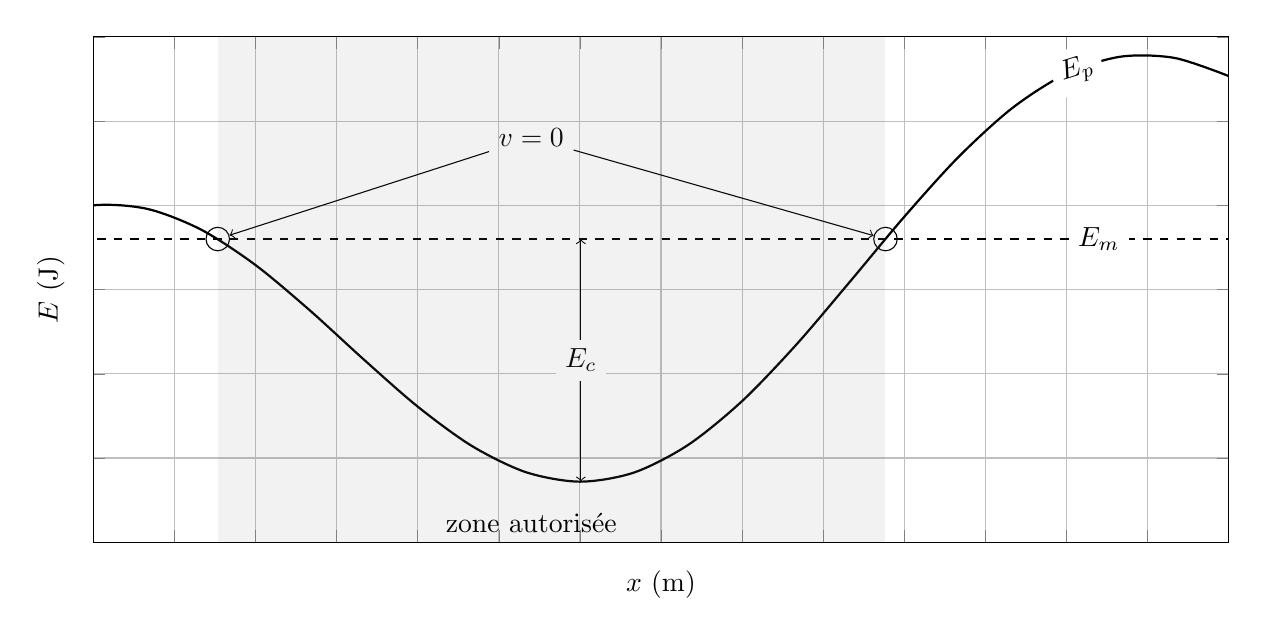
\begin{tikzpicture}
  %tikz meca
  \begin{axis}[
  width=16cm,
  height=8cm,
  xticklabels=\empty,
  yticklabels=\empty,
  xlabel=$x$ (m),
  ylabel=$E$ (J),
  xmin=0, xmax=7,
  ymin=-1, ymax=2,
  grid=both,
  xlabel near ticks,
  ylabel near ticks,
  ]
    \addplot[thick,domain=-1:7, smooth] {cos(deg(x)) + exp(x/10) -1} node[pos=0.9, sloped, fill=white]{$E_p$} ;
    \addplot[thick, dashed, domain=-1:7] {0.8} node[pos=0.9, fill=white]{$E_m$ };
    \draw (axis cs:0.767, 0.8) node[inner sep=3pt, draw, circle] (A){};
    \draw (axis cs:4.884, 0.8) node[inner sep=3pt, draw, circle] (B){};

    \draw[<->] (axis cs:3.006, -0.64) -- (axis cs:3.006, 0.8) node[midway, fill=white]{$E_c$};
    \draw (axis cs:2.7, 1.4) node(C) {$v=0$ };
    \draw[<-] (A) -- (C);
    \draw[<-] (B) -- (C);
    \fill[opacity=0.1, gray] (axis cs: 0.767, -1) rectangle (axis cs:4.884, 2);
    \draw (axis cs:2.7, -1) node[above]{zone autorisée};
  \end{axis}
\end{tikzpicture}
\end{center}
Dans cette configuration, le point matériel est confiné à la zone où $E_p<E_m$ car l'énergie cinétique est forcément positive. Le mouvement est périodique, le portrait de phase est une courbe fermée.


\begin{center}
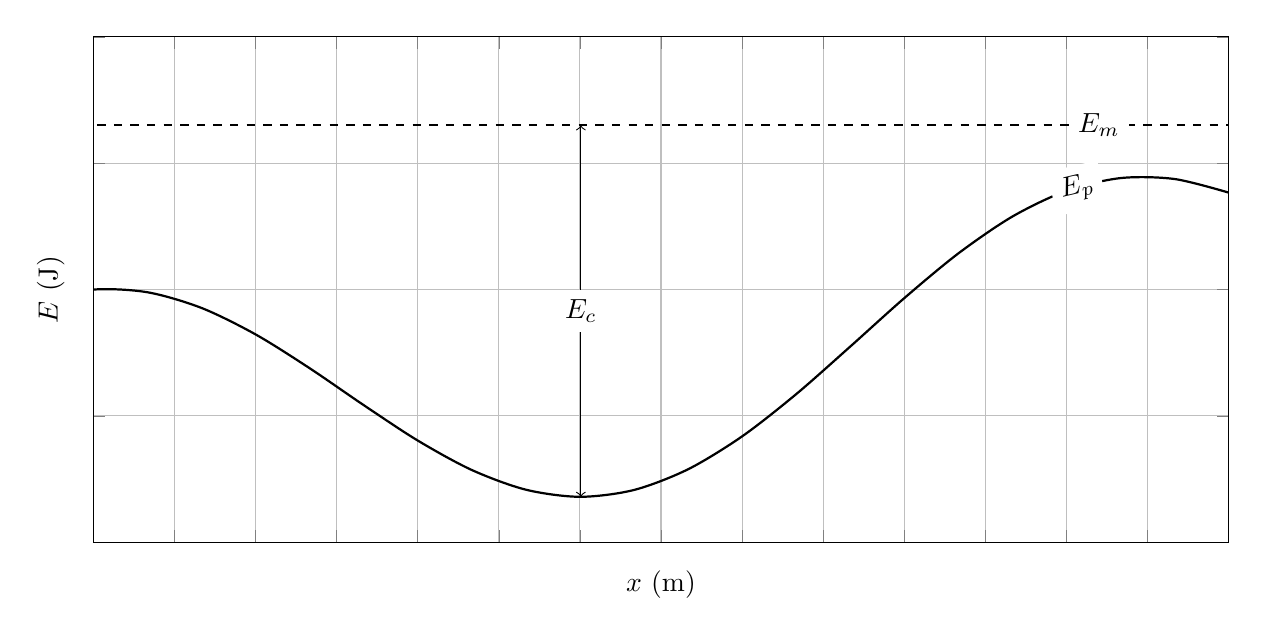
\begin{tikzpicture}
  %tikz meca
  \begin{axis}[
  width=16cm,
  height=8cm,
  xticklabels=\empty,
  yticklabels=\empty,
  xlabel=$x$ (m),
  ylabel=$E$ (J),
  xmin=0, xmax=7,
  ymin=-1, ymax=3.0,
  grid=both,
  xlabel near ticks,
  ylabel near ticks,
  ]
    \addplot[thick,domain=-1:7, smooth] {cos(deg(x)) + exp(x/10) -1} node[pos=0.9, sloped, fill=white]{$E_p$} ;
    \addplot[thick, dashed, domain=-1:7] {2.3} node[pos=0.9, fill=white]{$E_m$ };
    \draw[<->] (axis cs:3.006, -0.64) -- (axis cs:3.006, 2.3) node[midway, fill=white]{$E_c$};
  \end{axis}
\end{tikzpicture}
\end{center}
Si on donne suffisamment d'énergie mécanique au point matériel, toutes les positions sont autorisées, le mouvement du point matériel n'est pas borné, le mouvement n'est pas périodique et le portrait de phase est une courbe qui ne se referme pas.

\subsection{Équilibre et stabilité}%
\label{sub:equilibre_et_stabilite}

\subsubsection{Positions d'équilibre}%
\label{ssub:positions_d_equilibre}



Une position d'équilibre est une position pour laquelle $\vv{a}=\vv{0}$ donc $\sum \vv*{F}{i} = \vv{0}$. 

Considérons un point matériel $M$ soumis à une force conservative $\vv{F}$, l'énergie potentielle associée à $\vv{F}$ est $E_p$. Pour un petit déplacement $\D x$ du point $M$, on a
\begin{equation}
F\cdot \D x = E_p(x) - E_p(x + \D x) \Leftrightarrow F = -\frac{E_p(x+\D x)-E_p(x)}{\D x} =  -\frac{\D E_p}{\D x}
\end{equation}

Donc une position d'équilibre est caractérisée par $F=0$, soit

\begin{empheq}[box=\tcbhighmath]{equation*}
\frac{\D E_p}{\D x} = 0
\end{empheq}
Les positions d'équilibre sont les extrema locaux (maximum ou minimum) d'énergie potentielle.

On dit qu'une position d'équilibre est \textbf{stable} si la force subie par le point autour de la position d'équilibre tend à le ramener vers sa position d'équilibre. On doit donc avoir
\begin{itemize}
  \item $F(x+\D x) > 0$ si $\D x<0$ 
  \item $F(x+\D x) < 0$ si $\D x>0$ 
\end{itemize}
Soit
\begin{equation}
\frac{F(x+\D x)}{\D x} < 0 \Leftrightarrow \frac{F(x+\D x) - \overbrace{F(x)}^{=0}}{\D x} < 0 \Leftrightarrow \frac{\D F}{\D x}<0
\end{equation}
et comme on a vu que $F = -\frac{\D E_p}{\D x}$ on obtient la condition d'\textbf{équilibre stable} :

\begin{empheq}[box=\tcbhighmath]{equation*}
\frac{\D^2 E_p}{\D x^2} > 0
\end{empheq}
Ce qui correspond à un minimum d'énergie potentiel. 

Une position d'équilibre \textbf{instable} est telle que 
\begin{empheq}[box=\tcbhighmath]{equation*}
\frac{\D^2 E_p}{\D x^2} < 0
\end{empheq}
il s'agit alors d'un maximum d'énergie potentielle.

\begin{center}
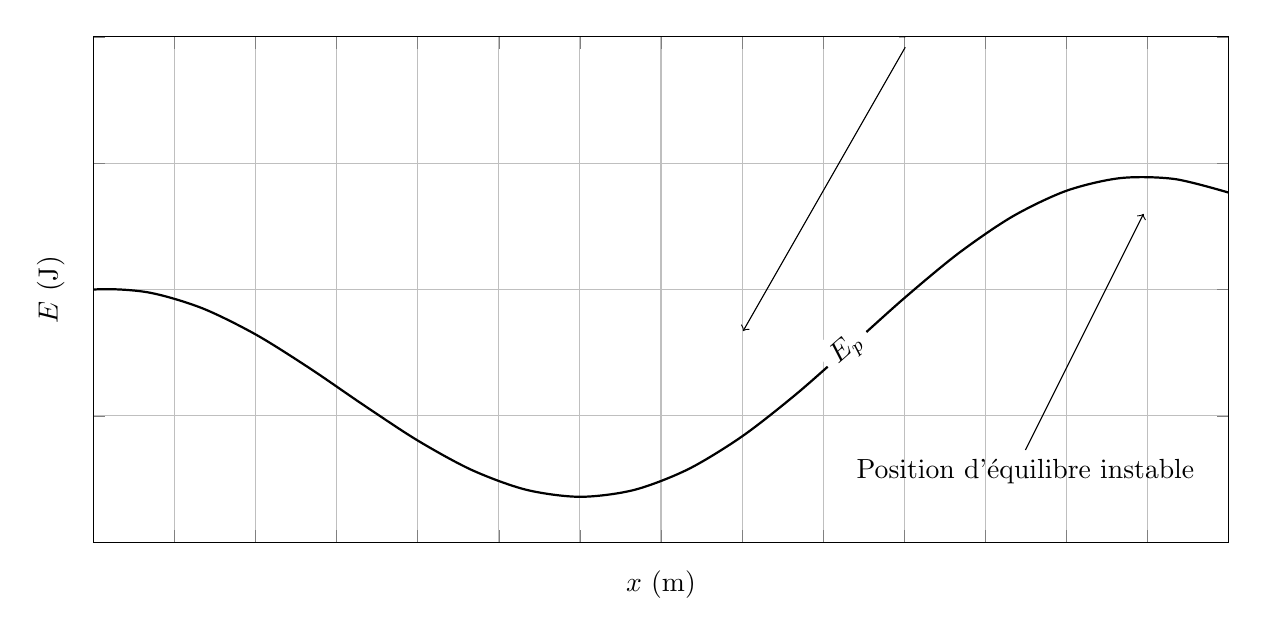
\begin{tikzpicture}
  \begin{axis}[
  width=16cm,
  height=8cm,
  xticklabels=\empty,
  yticklabels=\empty,
  xlabel=$x$ (m),
  ylabel=$E$ (J),
  xmin=0, xmax=7,
  ymin=-1, ymax=3.0,
  grid=both,
  xlabel near ticks,
  ylabel near ticks,
  ]
    \addplot[thick,domain=-1:7, smooth] {cos(deg(x)) + exp(x/10) -1} node[pos=0.7, sloped, fill=white]{$E_p$} ;
    \coordinate (A) at (axis cs:3.006, -0.64);
    \coordinate (B) at (axis cs:6.475, 1.6);
    \draw [<-] (A)  ++(0, 0.5cm) --  ++(0, 2cm) node[above] {Position d'équilibre stable};
    \draw [<-] (B) -- ++(-1.5cm, -3cm) node[below] {Position d'équilibre instable};
  \end{axis}
\end{tikzpicture}
\end{center}

\subsubsection{Mouvements autour d'une position d'équilibre}%
\label{ssub:mouvements_autour_d_une_position_d_equilibre}
Lorsqu'on écarte un point matériel d'une position d'équilibre stable, il va osciller autour de cette position.

Autour d'une position d'équilibre stable, on peut modéliser l'énergie potentielle par une parabole.

Si l'énergie potentielle présente un minimum en $x_0$, on peut la modéliser par une parabole autour de $x_0$ :
\begin{center}
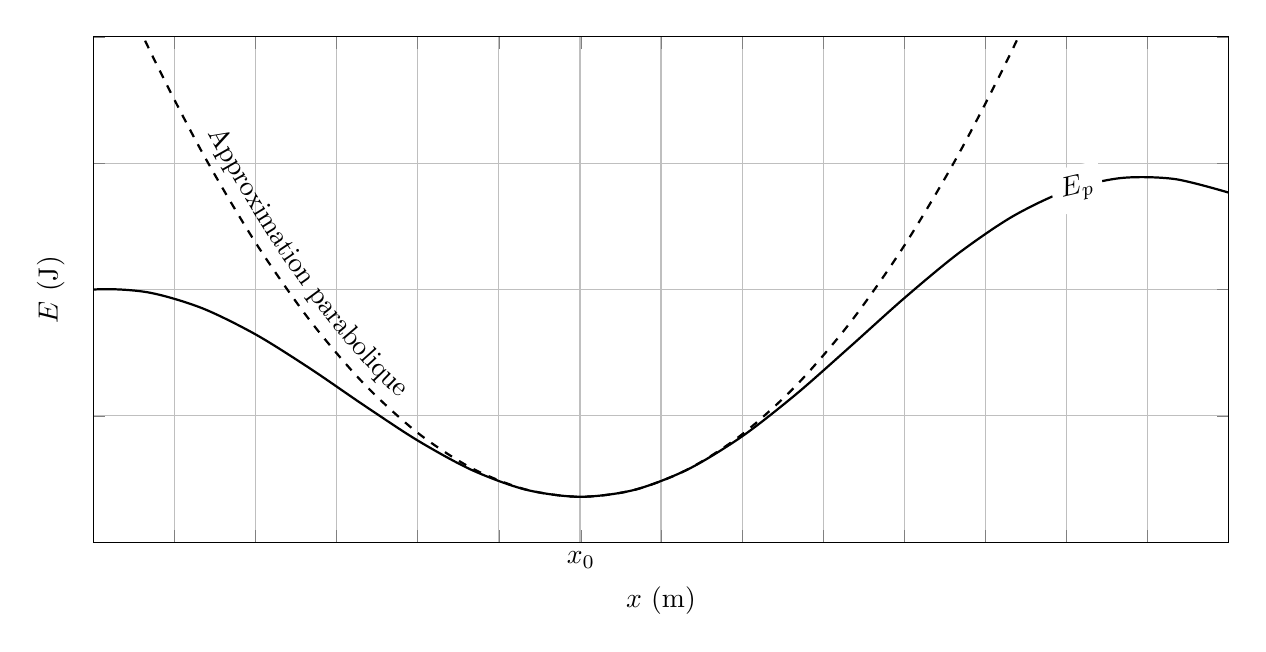
\begin{tikzpicture}
  %tikz meca
  \begin{axis}[
  width=16cm,
  height=8cm,
  xticklabels=\empty,
  yticklabels=\empty,
  extra x ticks={3.006},
  extra x tick labels={$x_0$},
  xlabel=$x$ (m),
  ylabel=$E$ (J),
  xmin=0, xmax=7,
  ymin=-1, ymax=3.0,
  grid=both,
  xlabel near ticks,
  ylabel near ticks,
  ]
    \addplot[thick,domain=-1:7, smooth] {cos(deg(x)) + exp(x/10) -1} node[pos=0.9, sloped, fill=white]{$E_p$} ;
    \addplot[thick, dashed, domain=-1:7, smooth, 
    decoration={
        raise=5pt,
        text along path,
        text={Approximation parabolique},
        text align={align=left, left indent=9cm},
    },
    postaction={decorate},
    ]
    {0.5*(x-3.006)^2-0.64} ;
    \coordinate (A) at (axis cs:3.006, -0.64);
    \coordinate (B) at (axis cs:6.475, 1.6);
  \end{axis}
\end{tikzpicture}
\end{center}

On cherche la parabole qui passe au plus près de la courbe. On sait déjà que son minimum se trouve en $x_0$ et vaut $E_p(x_0)$. L'équation de la parabole est donc de la forme :
\begin{equation}
f(x) = A(x-x_0)^2 + E_p(x_0)
\end{equation}
Il reste à trouver $A$. On veut que la \emph{courbure} de la parabole soit la même que celle de $E_p$ en $x_0$ . On veut donc 
\begin{equation}
\frac{\D^2 E_p}{\D x^2}(x_0) = \frac{\D^2 f}{\D x^2}(x_0) = 2A
\end{equation}
D'où 
\begin{equation}
A = \frac{1}{2}\frac{\D^2 E_p}{\D x^2}(x_0)
\end{equation}
 
On voit que si le point matériel s'écarte peu de sa position d'équilibre, son énergie potentielle est très proche de l'approximation parabolique. Déterminons le mouvement du point $M$. La conservation de l'énergie mécanique permet d'écrire :
\begin{equation}
E_m = E_c + E_p = \frac{1}{2}m \dot{x}^2 + A(x-x_0)^2 + E_p(x_0)
\end{equation}
On dérive cette équation par rapport à $x$
\begin{equation}
0 = m \dot{x} \ddot{x} + 2A(x-x_0)\dot{x} 
\end{equation}
En posant $x' = x-x_0$ le déplacement par rapport à la position d'équilibre et en divisant par $\dot{x}$ on obtient finalement
\begin{equation}
\ddot{x'} + \frac{2A}{m}x' = 0
\end{equation}
et on reconnait l'équation différentielle d'un \textbf{oscillateur harmonique} avec :
\begin{equation}
\omega_0^2 = \frac{2A}{m} = \frac{1}{m} \frac{\D^2 E_p}{\D x^2}
\end{equation}

On comprend pourquoi l'oscillateur harmonique est si important en physique, dès qu'un système oscille autour de sa position d'équilibre, on peut faire l'approximation parabolique de l'énergie potentielle et on a un comportement d'oscillateur harmonique.


\end{document}
